\documentclass{beamer}
 \mode<presentation>{ 
 \usetheme{Boadilla}%\usetheme{Warsaw}  
\setbeamercovered{invisible}
%   \usecolortheme{albatross} % for inverted color
% \usecolortheme{wolverine} % way too flashy!
\usecolortheme{beaver}

 } 
\usepackage[utf8]{inputenc}
\usepackage{listings} % For code examples
\usepackage{xcolor}

\usepackage{tikz-dependency} % For dependency trees
\usepackage{forest} % For phrase structure trees

\title{Introduction to Computational Linguistics and Natural Language Processing}
\author{Miquel Esplà-Gomis}
\date{November 25, 2026}

\AtBeginSection[]
{
  \begin{frame}<beamer>{Índex}
        \tableofcontents[hidesubsections,currentsection,currentsubsection]
  \end{frame}
}

\AtBeginSubsection[]
{
  \begin{frame}<beamer>{Índex}
        \tableofcontents[hidesubsections,currentsection,currentsubsection]
  \end{frame}
}

\DeclareUnicodeCharacter{0301}{\'{ }}

\begin{document}

\frame{\titlepage}

\begin{frame}{Presentation}
    \begin{itemize}
        \item Welcome to \alert{Natural Language Processing Techniques}
        \item Two teachers from the \textit{Department of Software and Computing Systems}:
        \begin{itemize}
            \item \textbf{Miquel Esplà Gomis} (myself): first session
            \item Juan Antonio Pérez Ortiz: rest of sessions
        \end{itemize}
        \item All the information is on the subject website: \url{https://mespla.github.io/tpln2627/}
        \item Attending classes:
        \begin{itemize}
          \item It is mandatory and we will take attendance
          \item It is allowed to miss one session without a justification
        \end{itemize}
     \end{itemize}
\end{frame}

\begin{frame}{Evaluation}
    \begin{itemize}
        \item All the information is available on the official teaching guide: \url{https://cvnet.cpd.ua.es/Guia-Docente/GuiaDocente/Index?wlengua=en&wcodasi=43505&scaca=2025-26}
        \item Three elements in evaluation:
        \begin{itemize}
          \item Practical activities at class (that you may need to complete at home): \alert{25\%}
          \item Tests on the materials you prepare before class : \alert{5\%}
          \item Final test on January the 18th : \alert{70\%}
        \end{itemize}
     \end{itemize}
\end{frame}

\section{Introduction}

\begin{frame}{Computational Linguistics (CL)}
    \begin{itemize}
        \item An interdisciplinary field at the intersection of:
        \begin{itemize}
            \item Linguistics
            \item Computer Science
        \end{itemize}
        \item Focuses on modeling human language using computational methods.
        \item Key objectives:
        \begin{itemize}
            \item Analyze and understand natural language.
            \item Develop linguistic theories supported by computational tools.
        \end{itemize}
        \item Example topics:
        \begin{itemize}
            \item Parsing syntactic structures.
            \item Phonetics and phonology modeling.
        \end{itemize}
    \end{itemize}
\end{frame}

\begin{frame}{Natural Language Processing (NLP)}
    \begin{itemize}
        \item A subfield of Artificial Intelligence (AI) and Machine Learning (ML).
        \item Focuses on designing algorithms and systems to process natural language data.
        \item Key objectives:
        \begin{itemize}
            \item Automate language-based tasks.
            \item Enable machines to interact with humans through language.
        \end{itemize}
        \item Example applications:
        \begin{itemize}
            \item Machine Translation (e.g., Google Translate).
            \item Sentiment Analysis.
            \item Question Answering Systems.
        \end{itemize}
    \end{itemize}
\end{frame}

\begin{frame}{Differences Between CL and NLP}
    \begin{itemize}
        \item \textbf{Computational Linguistics (CL):}
        \begin{itemize}
            \item Emphasizes theoretical understanding of language.
            \item Grounded in linguistic principles.
        \end{itemize}
        \item \textbf{Natural Language Processing (NLP):}
        \begin{itemize}
            \item Focuses on practical applications of language processing.
            \item Driven by engineering and computational efficiency.
        \end{itemize}
    \end{itemize}
\end{frame}

\begin{frame}{Commonalities Between CL and NLP}
    \begin{itemize}
        \item Both fields deal with natural language data.
        \item Share methods and tools, such as:
        \begin{itemize}
            \item Syntax and semantics modeling.
            \item Statistical and machine learning techniques.
        \end{itemize}
        \item Work towards improving human-computer interaction through language.
    \end{itemize}
\end{frame}


\begin{frame}{What will we talk about during this session?}
    \begin{itemize}
        \item \textbf{Text preprocessing}: preparing text for NLP applications
        \item \textbf{Morphological parsing}: how much information can we extract from words to better understanding text?
        \item \textbf{Syntactic parsing}: and what about the structure of the words in a sentence?
        \item \textbf{Vector representations of text}: how can we feed text in models that build on math?
    \end{itemize}
\end{frame}

\section{Text preprocessing}

\begin{frame}{Text Preprocessing: An Essential Step}
    \begin{itemize}
        \item Text preprocessing prepares raw text for effective processing by algorithms and models.
        \item Ensures consistency, reduces noise, and optimizes data for downstream tasks.
        \item Different tasks require different preprocessing steps.
    \end{itemize}
\end{frame}

\begin{frame}{Some frequent sub-tasks in Text Preprocessing}
    \begin{itemize}
        \item \textbf{Format Cleaning:}
        \begin{itemize}
            \item Remove unwanted formatting, such as HTML tags or PDF metadata.
        \end{itemize}
        \item \textbf{Text Tokenization:}
        \begin{itemize}
            \item Split text into smaller units like sentences, words, subwords, or characters.
        \end{itemize}
        \item \textbf{Text Normalization:}
        \begin{itemize}
            \item Normalize punctuation and spaces.
            \item Convert text to lowercase for case-insensitive processing.
        \end{itemize}
        \item \textbf{Dealing with Punctuation:}
        \begin{itemize}
            \item Remove or retain punctuation depending on the application.
        \end{itemize}
        \item \textbf{Identifying Stopwords:}
        \begin{itemize}
            \item Remove commonly used words (e.g., \textit{the}, \textit{is}, \textit{and}) to focus on meaningful content.
        \end{itemize}
    \end{itemize}
\end{frame}

\subsection{Removing Formatting}

\begin{frame}{Why do we need to clean format?}
    \begin{itemize}
        \item Raw text often comes in formats unsuitable for NLP models:
        \begin{itemize}
            \item HTML files with tags and scripts.
            \item PDF documents with metadata and layout information.
            \item Markdown files with format marks.
        \end{itemize}
        \item In most cases data related to format adds noise to the text to be processed.
    \end{itemize}
\end{frame}

\begin{frame}{Removing Formatting: HTML and PDF}
    \begin{itemize}
        \item \textbf{HTML:}
        \begin{itemize}
            \item Often contains tags (\texttt{<div>}, \texttt{<script>}, etc.) and styles.
            \item Content extraction involves ignoring these elements.
        \end{itemize}
        \item \textbf{PDF:}
        \begin{itemize}
            \item May include page numbers, headers, and images.
            \item Text extraction tools can help retrieve only textual content.
        \end{itemize}
    \end{itemize}
\end{frame}

\begin{frame}[fragile]{Example: Removing HTML Tags}
    \textbf{Raw Text:}
     \begin{lstlisting}[basicstyle=\ttfamily\small,backgroundcolor=\color{gray!10}]
 <html>
     <head><title>Example</title></head>
     <body>
         <h1>Hello, World!</h1>
         <p>This is a sample text.</p>
     </body>
 </html>
     \end{lstlisting}

     \vspace{1em}
     \textbf{Cleaned Text:}
    \begin{lstlisting}[basicstyle=\ttfamily\small,backgroundcolor=\color{gray!10}]
Hello, World!
This is a sample text.
    \end{lstlisting}
\end{frame}

\begin{frame}{Techniques for Removing Formatting}
    \begin{itemize}
        \item Regular Expressions (Regex):
        \begin{itemize}
            \item Use patterns to identify and remove unwanted elements.
            \item Example: Remove HTML tags using the pattern \texttt{<.*?>}.
        \end{itemize}
        \item Libraries and Tools:
        \begin{itemize}
            \item \texttt{BeautifulSoup} (Python): For parsing and cleaning HTML.
            \item \texttt{PyPDF2} (Python): For extracting text from PDFs.
        \end{itemize}
        \item OCR Tools:
        \begin{itemize}
            \item Use Optical Character Recognition for images or scanned text.
        \end{itemize}
    \end{itemize}
\end{frame}

\begin{frame}{Common Challenges in Formatting Removal}
    \begin{itemize}
        \item Handling noisy or incomplete data.
        \item Retaining meaningful structure (e.g., tables, paragraphs).
        \item Managing large or complex files efficiently.
        \item Language-specific formatting (e.g., RTL scripts or special characters).
    \end{itemize}
\end{frame}

\subsection{Tokenization}

\begin{frame}{What is Tokenization?}
    \begin{itemize}
        \item The process of breaking text into smaller units, called \textbf{tokens}.
        \item Tokens can represent:
        \begin{itemize}
            \item Sentences (it is also usual to call this task \textit{sentence splitting})
            \item Words
            \item Characters
            \item Sub-words
        \end{itemize}
        \item Critical for transforming raw text into a format suitable for NLP algorithms.
    \end{itemize}
\end{frame}

\begin{frame}{Levels of Tokenization}
    \begin{itemize}
        \item \textbf{Sentence Tokenization:}
        \begin{itemize}
            \item Splits text into sentences.
            \item Example: \textit{“NLP is fascinating. Tokenization is essential.”}
            \item Tokens: \textit{[“NLP is fascinating.”, “Tokenization is essential.”]}
        \end{itemize}
        \item \textbf{Word Tokenization:}
        \begin{itemize}
            \item Splits text into words.
            \item Example: \textit{“NLP is fascinating”}
            \item Tokens: \textit{[“NLP”, “is”, “fascinating”]}
        \end{itemize}
        \item \textbf{Character Tokenization:}
        \begin{itemize}
            \item Splits text into individual characters.
            \item Example: \textit{“NLP”}
            \item Tokens: \textit{[“N”, “L”, “P”]}
        \end{itemize}
        \item \textbf{Sub-word Tokenization:}
        \begin{itemize}
            \item Splits words into potentially meaningful sub-units.
            \item Example: \textit{“unbelievable”}
            \item Tokens: \textit{[“un”, “believ”, “able”]}
        \end{itemize}
    \end{itemize}
\end{frame}


\begin{frame}{Sentence splitting}
    \begin{itemize}
        \item For most languages, \textbf{punctuation} is used (split by colons, semicolons, etc.)
        \begin{itemize}
            \item This is sometimes difficult: "\textit{This is Dr. Smith. He is the author of the blog \texttt{saludparatodos.net}.}"
        \end{itemize}
        \item Sometimes it is possible to use \textbf{format};for example, some HTML tags delimit a text block, such as \texttt{<p>} or \texttt{<h1>}

        \item \textbf{Some languages do not use punctuation} (Thai, for example)

        \vspace{0.3cm}
        
        
\includegraphics[width=0.90\textwidth]{img/thai.png}
    \end{itemize}
\end{frame}

\begin{frame}{Word Tokenization Strategies}
    \begin{itemize}
        \item \textbf{Whitespace-Based Tokenization:}
        \begin{itemize}
            \item Fails with contractions or punctuation, for example.
            \item Words separated with a dash in English: \textit{state-of-the-art}.
            \item What to do with languages that don't use spaces to separate words?
        \end{itemize}
        
        \item \textbf{Using regular expressions:}
        \begin{itemize}
            \item Allows to identify some phenomena: some contractions in English, URLs, etc.
        \end{itemize}
        \item \textbf{Language-Specific Tokenizers:} Tailored to account for language-specific features.
        \begin{itemize}
            \item Example: Tokenizing Japanese using MeCab or SudachiPy.
            \item There are tokenizers that build on knowledge (morphological dictionaries) and that build on statistical models (for example, HMM).
        \end{itemize}
    \end{itemize}
\end{frame}

\begin{frame}{Why Sub-word Tokenization?}
    It has become very popular in neural-based NLP models:
    \begin{itemize}
        \item Addresses issues with \textbf{rare words} and \textbf{out-of-vocabulary} (OOV) words.
        \item Efficient for \textbf{morphologically rich languages}.
        \item Maintains a balance between word and character tokenization.
    \end{itemize}
\end{frame}

\begin{frame}{Approaches to Sub-word Tokenization}

    Task traditionally based on \textbf{morphological segmentation}.

    \vspace{1cm}

    \textbf{Two popular strategies in the neural age:}
    \begin{itemize}
        \item Byte Pair Encoding (BPE)
        \item Unigram Language Model
    \end{itemize}
\end{frame}

\begin{frame}{Byte Pair Encoding (BPE)}
    \begin{itemize}
        \item Begins by splitting text in characters.
        \item Iteratively merges the most frequent pairs of characters or subwords.
        \item Example:
        \begin{itemize}
            \item Initial tokens: \texttt{["l", "o", "w", "e", "r"]}
            \item Merge "l" and "o" → \texttt{["lo", "w", "e", "r"]}
            \item Merge "lo" and "w" → \texttt{["low", "e", "r"]}
        \end{itemize}
        \item Benefits:
        \begin{itemize}
            \item Handles rare words by breaking them into sub-units.
            \item Compact vocabulary size.
        \end{itemize}
    \end{itemize}
\end{frame}

\begin{frame}{Unigram Language Model}
    \begin{itemize}
        \item Steps:
        \begin{itemize}
            \item Start with a large vocabulary of potential subwords (could be all the possible sub-words in the corpus).
            \item Assign a probability to each of them according to their frequency observed in the corpus.
            \item Use the vocabulary as an unigram model that allows to obtain the probability of a word.
            \item Iteratively remove subwords that minimally impact the overall probability of the corpus.
        \end{itemize}
        \item Benefits:
        \begin{itemize}
            \item Allows for multiple segmentations with probabilities.
            \item More flexible than deterministic methods like BPE.
        \end{itemize}
    \end{itemize}
\end{frame}

\begin{frame}{Comparison: BPE vs. Unigram}
    \begin{itemize}
        \item \textbf{BPE:}
        \begin{itemize}
            \item Deterministic.
            \item Fixed segmentation after training.
        \end{itemize}
        \item \textbf{Unigram:}
        \begin{itemize}
            \item Probabilistic.
            \item Allows multiple valid segmentations with probabilities.
        \end{itemize}
        \item \textbf{In common:}
        \begin{itemize}
            \item Both require pre-tokenization.
            \item Both allow to specify the size of the final vocabulary.
        \end{itemize}
        
    \end{itemize}
\end{frame}

\begin{frame}{SentencePiece}
    \begin{itemize}
      \item It builds on Unigram or BPE
      \item Unigram and BPE assume that the corpus can be split in words by blank spaces.
      \item SentencePiece just omits this assumption:
      \begin{itemize}
          \item Includes spaces in the initial vocabulary of BPE.
          \item Includes sub-words containing spaces in the initial vocabulary of Unigram.
      \end{itemize}
      \item Allows dealing with languages that do not use blank spaces.
      \item Allows using multi-word expressions as elements in the final vocabulary.
    \end{itemize}
\end{frame}
\subsection{Text normalization}


\begin{frame}{What is Text Normalization?}
    \begin{itemize}
        \item The process of converting text into a standard form.
        \item Aims to reduce variability in the text while preserving meaning.
        \item Prepares text for consistent and effective processing in NLP tasks.
    \end{itemize}
    \vspace{1em}
    \textbf{Examples:}
    \begin{itemize}
        \item \textit{“Hello,”} → \textit{“hello”} (lowercasing).
        \item \textit{“I’ve got 2 apples.”} → \textit{“i have two apples”} (normalizing contractions and numbers).
    \end{itemize}
\end{frame}

\begin{frame}{Challenges with Unicode Characters}
    \begin{itemize}
        \item Modern text is usually encoded with \textbf{Unicode} that support a wide variety of scripts. Sometimes this leads to data sparsity at character level.
        \item \textbf{Visually Similar Characters:}
        \begin{itemize}
            \item \texttt{“á” (U+00E1)} vs. \texttt{“á” (U+0061 + U+0301)}.
            \item Appear identical but have different underlying representations.
            \item With punctuation it is even worse; have a look to UTF-8 punctuation at: \url{https://www.compart.com/en/unicode/category/Po}
        \end{itemize}
        \item \textbf{Non-breaking Spaces and Invisible Characters:}
        \begin{itemize}
            \item \texttt{“ ” (non-breaking space, U+00A0)} vs. \texttt{“ ” (space, U+0020)}.
            \item Introduce subtle errors in processing.
        \end{itemize}
    \end{itemize}
\end{frame}

\begin{frame}{Task-Specific Normalization Needs}

    \begin{itemize}
        \item Text normalization varies depending on the NLP task.
        \item \textbf{Examples:}
        \begin{itemize}
            \item \textbf{Case-sensitive tasks:}
            \begin{itemize}
                \item Named Entity Recognition (NER): Retain original casing to identify entities like \textit{“Apple”}.
            \end{itemize}
            \item \textbf{Removing Punctuation:}
            \begin{itemize}
                \item Useful for bag-of-words models.
                \item Not always suitable for tasks like sentiment analysis.
            \end{itemize}
            
            \item \textbf{Removing redundant text:}
            \begin{itemize}
                \item Removing duplicate or almost-duplicate sentences or paragraphs in a long corpus.
                \item Useful when we have a large corpus to training generative models. 
            \end{itemize}
            
        \end{itemize}
        \item Normalization must strike a balance between generality and task-specific requirements.
    \end{itemize}
\end{frame}

\begin{frame}{Summary of Text Normalization}
    \begin{itemize}
        \item Essential for standardizing text and reducing variability.
        \item Unicode introduces challenges like visually similar characters and non-breaking spaces.
        \item Techniques include lowercasing, punctuation removal, and whitespace normalization.
        \item Task-specific normalization must be tailored to the application.
    \end{itemize}
    \vspace{1em}
    \textbf{Key Takeaway:} Effective normalization improves downstream NLP performance.
\end{frame}


\subsection{Stopwords}

\begin{frame}
\frametitle{What are Stopwords?}
Stopwords are common words that are consider to contain low semantic value and are removed during text preprocessing for some NLP tasks.

\begin{itemize}
    \item Examples: "the", "is", "in", "on", "at", "and", "for"
    \item Removing them can improve efficiency and focus on more important words
    \item They are more usual in languages with low morpholocial complexity.
\end{itemize}
\end{frame}

\begin{frame}
\frametitle{How to Detect Stopwords}
Stopwords can be detected in various ways:

\begin{itemize}
    \item Predefined stopword lists (e.g., NLTK, SpaCy)
    \item Frequency-based approaches: 
        \begin{itemize}
            \item Words appearing very frequently across many documents are potential stopwords
            \item Commonly occurring words across corpora are candidates
        \end{itemize}
    \item Part-of-speech tagging: 
        \begin{itemize}
            \item Function words (e.g., determiners, prepositions, conjunctions) are often stopwords
        \end{itemize}
\end{itemize}
\end{frame}

\begin{frame}{Vocabulary frequency distribution}
            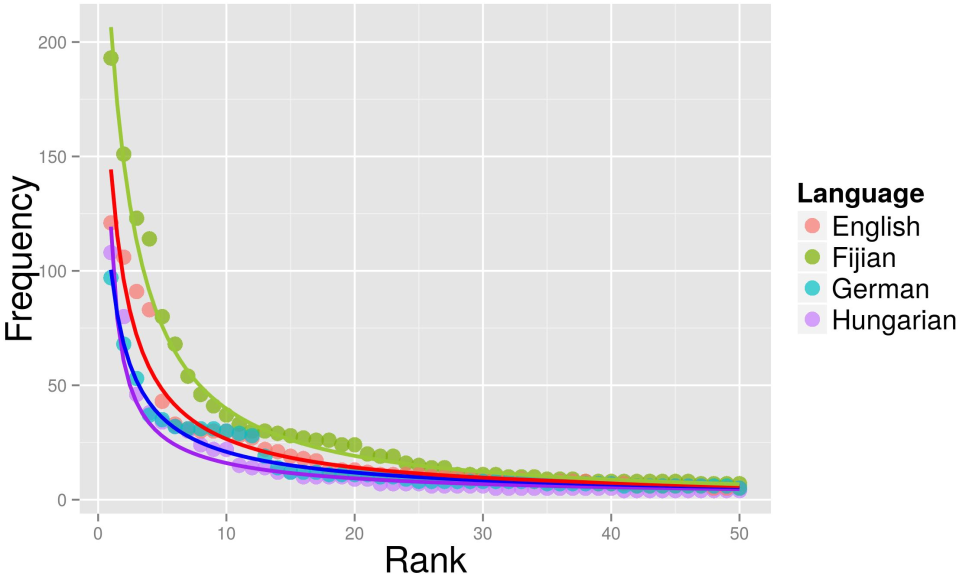
\includegraphics[width=\textwidth]{img/zipf_languages.png}
\small Figure 2 from: Bentz, C., Verkerk, A., Kiela, D., Hill, F., \& Buttery, P. (2015). \textbf{Adaptive communication: Languages with more non-native speakers tend to have fewer word forms}. \textit{PloS one}, 10(6).
\end{frame}


\begin{frame}
\frametitle{The zipfian distribution of vocabulary}

\begin{itemize}
    \item When the words in a corpus are ranked decreasingly they follow a zipfian distribution in which:
    \[
      \mathrm{freq}(r) \propto \frac{1}{r}
    \]
    \item In other words:
    \begin{itemize}
        \item a few words in most languages have a very high frequency, and
        \item most of the words in a language are in the so called "long tail".
    \end{itemize}
    \item The most frequent words in a language are typically function words (stopwords)
\end{itemize}
\end{frame}


\begin{frame}
\frametitle{Implications of Removing Stopwords in NLP}

Removing stopwords has several effects:

\begin{itemize}
    \item \textbf{Focuses on meaningful terms:} It can help to emphasize content-bearing words for tasks like classification or clustering
    \item \textbf{Risk of losing context:} Removing too many stopwords may change the sentence structure and meaning
    \item \textbf{Task-specific considerations:} Some tasks (e.g., sentiment analysis, language modeling, etc.) may benefit from retaining stopwords
\end{itemize}
\end{frame}

\section{Morphological parsing}

% Slide 1: Introduction
\begin{frame}{What is Morphological Parsing?}
    \begin{itemize}
        \item \textbf{Morphology}: Study of the structure of words.
        \item \textbf{Morphological Parsing}: Breaking down words into:
        \begin{itemize}
            \item \textbf{Lemmas}: Base forms of words.
            \item \textbf{Morphemes}: Smallest units of meaning (roots, prefixes, suffixes).
        \end{itemize}
        \item Essential for understanding word formation, meaning, and grammatical roles.
    \end{itemize}
\end{frame}

% Slide 2: Why is Morphological Parsing Important?
\begin{frame}{Why is Morphological Parsing Important?}
    \begin{enumerate}
        \item \textbf{Handling Rich Morphology}:
        \begin{itemize}
            \item Languages like Finnish, Turkish, or Arabic have complex word structures.
        \end{itemize}
        \item \textbf{Vocabulary Reduction}:
        \begin{itemize}
            \item Groups inflected forms (e.g., \textit{run}, \textit{ran}, \textit{running}) into a single base form.
        \end{itemize}
        \item \textbf{Text Normalization}:
        \begin{itemize}
            \item Preprocessing for tasks like sentiment analysis and information retrieval.
        \end{itemize}
    \end{enumerate}
\end{frame}

\begin{frame}{Most languages in Europe have rather simple morphology}
 We are used to \textbf{fusional languages}: few inflectional morphemes that add information to a stem.
  \begin{exampleblock}{A word in English}
     \textbf{Computed}
  \end{exampleblock}

\vspace{1cm}

  \begin{tabular}{ccccccccc}
  Comput & ed \\
  Setm & suffix indicating past \\
  \end{tabular}

 
\end{frame}


\begin{frame}{How complex can morphology get? 1/}
 There are also \textbf{agglutinative languages}: combine many inflectional morphemes each of them adding new information.
  \begin{exampleblock}{A word in Finnish}
     \textbf{Taloissammekin}
  \end{exampleblock}

\vspace{1cm}

  \begin{tabular}{ccccc}
  talo & i & ssa & mme & kin \\
  house & PLURAL & INNESIVE CASE & our & also \\
  
  \end{tabular}

 
\end{frame}

\begin{frame}{How complex can morphology get? 2/}
And then, there are \textbf{polysynthetic languages}, that put many words together.
  \begin{exampleblock}{A word in Inuktitut}
     \textbf{annulaksikkanninginnajualugasulauqsimagumanngittsiaqgaluaqtunga}
  \end{exampleblock}

\vspace{1cm}

  \begin{tabular}{ccccccccc}
  annulaksi & kkanni & nginna & jualu & gasu & lauqsima & guma & nngit & ... \\
  imprison & again & really &a lot & try &ever &want & NEG & ... \\
  \end{tabular}

\vspace{1cm}
  
\textit{I would never ever even want to try to end up in jail ever again even for a bit.}
(Johns, 2007)
 
\end{frame}
\begin{frame}{Why is important morphology in the age of neural technologies?}
    Two main uses:
    \begin{itemize}
        \item \textbf{In NLP}: mostly useful for low-resource languages
        \begin{itemize}
            \item Simplifies text (helps to segment words).
            \item Extracts information relevant to understand meaning.
            \item Generation morphologically-correct text.
            \item Support for language learners.
        \end{itemize}
        \item \textbf{In CL}:
        \begin{itemize}
            \item Automatic annotation of corpora.
            \item Supports linguists in discovering linguistic phenomena.
        \end{itemize}
    \end{itemize}
\end{frame}



% Slide 4: Modern NLP and Morphology
\begin{frame}{Relevant resources for morphology in NLP 1/}
    \begin{itemize}
        \item \textbf{Unimorph}: Datasets with exhaustive lists of words in 169 languages with tuples consisting of lemmas, surface words, word segmentation and lexical information (PoS, number, gender, case, etc.)
        \item \textbf{Universal Dependencies}: Corpora with (among other information) words are annotated with the lemma, the PoS and additional lexical information.
    \end{itemize}
\end{frame}

\begin{frame}{Unimorph}
    Provides type-level annotation, and is more exhaustive (is likelier to cover more words of a language.

    \begin{center}
        
    \begin{tabular}{l|l|l}
      \textbf{lemma} & \textbf{surface form} & \textbf{lex. info} \\ \hline
      eat	  & eats         & V;PRS;3;SG \\
      eat   & eating       & V;V.PTCP;PRS \\
      eat   & ate          & V;PST \\
      eat   & eaten        & V;V.PTCP;PST \\
      eat   & eats         & N;PL
    \end{tabular}
    \end{center}
\end{frame}

\begin{frame}{Universal Dependences}
    Provides \textbf{token-level annotation} with tokens in a context.

    \begin{center}
        
   \begin{tabular}{l|l|l|l}
Form       & Lemma     & PoS & lex. info   \\
\hline
He         & he        & PRON & PERS-P3SG-NOM  Case=Nom... \\
ate        & eat       & VERB & PAST           Mood=Ind|Tense=Past... \\
a          & a         & DET  & IND-SG         Definite=Ind... \\
mouthful   & mouthful  & NOUN & SG-NOM        Number=Sing     \\
\end{tabular}
    \end{center}
\end{frame}




\section{Syntactic parsing}


% Slide 1: Introduction to Syntactic Parsing
\begin{frame}{What is Syntactic Parsing?}
    \begin{itemize}
        \item Syntactic parsing is aimed at determining the structure of a sentence.
        \item It provides representations that help understand relationships between words.
        \item Two main strategies:
        \begin{itemize}
            \item Phrase Structure (Constituency Grammar)
            \item Dependency Structure (Dependency Grammar)
        \end{itemize}
    \end{itemize}
\end{frame}

% Slide 2: Phrase Structure
\begin{frame}{Phrase Structure}
    \begin{itemize}
        \item Represents syntax as nested phrases.
        \item Commonly associated with constituency grammar.
    \end{itemize}
    \begin{forest}
        [S
            [NP
                [Det [The]]
                [N [boy]]
            ]
            [VP
                [V [saw]]
                [NP
                    [Det [a]]
                    [Adj [small]]
                    [N [dog]]
                ]
                [PP
                    [P [in]]
                    [NP
                        [Det [the]]
                        [N [park]]
                    ]
                ]
            ]
        ]
    \end{forest}
\end{frame}

% Slide 3: Dependency Structure
\begin{frame}{Dependency Structure}
    \begin{itemize}
        \item Represents syntax as directed relationships between words.
        \item Captures dependencies directly.
    \end{itemize}
    \begin{dependency}[theme=night]
        \begin{deptext}
            The \& boy \& saw \& a \& small \& dog \& in \& the \& park \\
        \end{deptext}
        \deproot{3}{root}
        \depedge{2}{1}{det}
        \depedge{3}{2}{nsubj}
        \depedge{3}{6}{obj}
        \depedge{6}{4}{det}
        \depedge{6}{5}{amod}
        \depedge{3}{7}{obl}
        \depedge{7}{8}{det}
        \depedge{7}{9}{nmod}
    \end{dependency}
\end{frame}

% Slide 4: Cross-Linguistic Applicability of Dependency Structure
\begin{frame}{Why Dependency Structure is More Universal}
    \begin{itemize}
        \item Dependency grammar focuses on word-to-word relations.
        \item Easier to apply to languages with different word orders (e.g., SVO, OVS, SOV, etc.).
    \end{itemize}
\end{frame}

% Slide 5: Example - SVO vs. OVS
\begin{frame}{Example: Syntax Analysis in Two Languages 1/}
    \textbf{English (SVO):} The priests read the books.\\

    \vspace{0.5cm}
\fboxsep=0pt
\noindent{%
\begin{minipage}[t]{0.54\linewidth}
\textbf{Phrase Structure:}

    \begin{forest}
        [S
            [NP [DET [The]] [N [priests]]]
            [VP
                [V [read]]
                [NP [DET [the]] [N [books]]]
            ]
        ]
    \end{forest}
    
\end{minipage}}%
\hfill{%
\begin{minipage}[t]{0.42\linewidth}
\textbf{Dependency Structure:}

    \begin{dependency}[theme=night]
        \begin{deptext}
            The \& priests \& read \& the \& books \\
        \end{deptext}
        \deproot{3}{root}
        \depedge{2}{1}{det}
        \depedge{3}{2}{nsubj}
        \depedge{3}{5}{obj}
        \depedge{5}{4}{det}
    \end{dependency}
\end{minipage}
}
\end{frame}

% Slide 5: Example - SVO vs. OVS
\begin{frame}{Example: Syntax Analysis in Two Languages 2/}
    \textbf{Irish (VSO):} Léann na sagairt na leabhair.\\

    \vspace{0.5cm}
\fboxsep=0pt
\noindent{%
\begin{minipage}[t]{0.54\linewidth}
\textbf{Phrase Structure:}

    \begin{forest}
        [S
            [VP
                [V [Léan]]
                [NP 
                  [NP [DET [na]] [N [sagairt]]]
                  [NP [DET [na]] [N [leabhair]]]
                ]
            ]
        ]
    \end{forest}
    
\end{minipage}}%
\hfill{%
\begin{minipage}[t]{0.42\linewidth}
\textbf{Dependency Structure:}

    \begin{dependency}[theme=night]
        \begin{deptext}
            Léann \& na \& sagairt \& na \& leabhair \\
        \end{deptext}
        \deproot{1}{root}
        \depedge{3}{2}{det}
        \depedge{1}{3}{nsubj}
        \depedge{1}{5}{obj}
        \depedge{5}{4}{det}
    \end{dependency}
\end{minipage}
}
\end{frame}

\begin{frame}{Why is important syntax in the age of neural technologies?}
    Two main uses:
    \begin{itemize}
        \item \textbf{In NLP}: mostly useful for low-resource languages
        \begin{itemize}
            \item Split text into meaningful fragments
            \item Disambiguate text
            \item Knowledge-enhanced models (summarization, translation, etc.)
            \item Helps identify named entities
        \end{itemize}
        \item \textbf{In CL}:
        \begin{itemize}
            \item Automatic annotation of corpora.
            \item Search of specific syntactic structures in corpora.
            \item Supports linguists in discovering linguistic phenomena.
        \end{itemize}
    \end{itemize}
\end{frame}


\begin{frame}{Universal Dependences}
    Annotation of both \textbf{morphological information} and \textbf{syntactic dependencies}

    \begin{center}
        \small
   \begin{tabular}{l|l|l|l|l|l}
Form       & Lemma     & PoS & lex. info & Dep. & Dep. type   \\
\hline
You      & you      & PRON & PERS-P2                & 3 & nsubj \\
can      & can      & AUX  & PRES-AUX VerbForm=Fin  & 3 & aux \\
change   & change   & VERB & INF VerbForm=Inf       & 0 & root \\
the      & the      & DET  & DEF Definite=Def       & 6 & det \\
security & security & NOUN & SG-NOM Number=Sing     & 6 & compound \\
mode     & mode     & NOUN & SG-NOM Number=Sing     & 3 & obj \\
... & ... & ... & ... & ... & ...\\
\end{tabular}
    \end{center}
\end{frame}

\begin{frame}{What tools can be used for dependency parsing?}
    Many tools. Some of the most popular ones:
    \begin{itemize}
        \item \textbf{Stanza}: 
        \begin{itemize}
            \item Graph-based parsing implemented as a neural network. 
            \item Multilingual from its inception.
            \item More exhaustive, also slower.
        \end{itemize}
        \item \textbf{ScyPy}:
        \begin{itemize}
            \item Statistical implementation of transition models.
            \item Initially focused on English, now it covers wide range of languages.
            \item More prone to make errors with long-range language phenomena, but faster.
        \end{itemize}
    \end{itemize}
\end{frame}

\section{Vector representations of text}



\begin{frame}{Words have meaning}
  \begin{block}{Semantic compositionality principle}
    The meaning of a \textbf{complex expression} (a sentence) is determined by the \textbf{meanings of its constituent parts} (words) and \textbf{the way they are combined} (syntax).
  \end{block}
  
    \begin{itemize}
        \item \textbf{Lexeme}: A unit of meaning in language, independent of inflectional forms.
        \begin{itemize}
            \item Example: The lexeme \textit{run} covers \textit{runs}, \textit{running}, \textit{ran}.
        \end{itemize}
        \item \textbf{Word Sense}: The specific meaning of a word in a given context.
        \begin{itemize}
            \item Example: \textit{bank} (financial institution) vs. \textit{bank} (riverbank).
        \end{itemize}
    \end{itemize}
\end{frame}

\begin{frame}{Words are related by their meaning}
  \begin{itemize}
      \item \textbf{Synonymy}: words mean (almost) the same 
      \item \textbf{Antonymy}: words are opposite
      \item \textbf{Similarity}: words share some aspects of their meaning
      \item \textbf{Relatedness}: words belong to the same \textit{semantic field}
      \item \textbf{Connotation}: connotations independent of the meaning (for example, sentiment)
  \end{itemize}
\end{frame}

\begin{frame}{Words are related by their meaning}
  \begin{itemize}
      \item \textbf{Synonymy}: words mean (almost) the same 
      \begin{itemize}
          \item \textit{big} and \textit{large}
          \item yes, but: \textit{my big sister} \textbf{!=} \textit{my large sister}
          \item \textbf{Linguistic principle of contrast}: different form $\rightarrow$ different meaning
      \end{itemize}
      \item \textcolor{gray}{\textbf{Antonymy}: words are opposite}
      \item \textcolor{gray}{\textbf{Similarity}: words share some aspects of their meaning}
      \item \textcolor{gray}{\textbf{Relatedness}: words belong to the same \textit{semantic field}}
      \item \textcolor{gray}{\textbf{Connotation}: connotations independent of the meaning (for example, sentiment)}
  \end{itemize}
\end{frame}

\begin{frame}{Words are related by their meaning}
  \begin{itemize}
      \item \textcolor{gray}{\textbf{Synonymy}: words mean (almost) the same }
      \item \textbf{Antonymy}: words are opposite
      \begin{itemize}
          \item \textit{big} vs. \textit{small}
          \item \textit{up} vs. \textit{down}
      \end{itemize}
      \item \textcolor{gray}{\textbf{Similarity}: words share some aspects of their meaning}
      \item \textcolor{gray}{\textbf{Relatedness}: words belong to the same \textit{semantic field}}
      \item \textcolor{gray}{\textbf{Connotation}: connotations independent of the meaning (for example, sentiment)}
  \end{itemize}
\end{frame}

\begin{frame}{Words are related by their meaning}
  \begin{itemize}
      \item \textcolor{gray}{\textbf{Synonymy}: words mean (almost) the same}
      \item \textcolor{gray}{\textbf{Antonymy}: words are opposite}
      \item \textbf{Similarity}: words share some aspects of their meaning
      \begin{itemize}
          \item \textit{cow}, \textit{horse} $\rightarrow$ ruminants, size, etc.
          \item \textit{pen}, \textit{pencil} $\rightarrow$ shape, purpose, etc.
      \end{itemize}
      \item \textcolor{gray}{\textbf{Relatedness}: words belong to the same \textit{semantic field}}
      \item \textcolor{gray}{\textbf{Connotation}: connotations independent of the meaning (for example, sentiment)}
  \end{itemize}
\end{frame}

\begin{frame}{Words are related by their meaning}
  \begin{itemize}
      \item \textcolor{gray}{\textbf{Synonymy}: words mean (almost) the same }
      \item \textcolor{gray}{\textbf{Antonymy}: words are opposite}
      \item \textcolor{gray}{\textbf{Similarity}: words share some aspects of their meaning}
      \item \textbf{Relatedness}: words belong to the same \textit{semantic field}
      \begin{itemize}
          \item \textit{coffee}, \textit{cup} $\rightarrow$ coffee is served in cups.
          \item \textit{car}, \textit{wheel} $\rightarrow$ cars have four wheels.
      \end{itemize}
      \item \textcolor{gray}{\textbf{Connotation}: connotations independent of the meaning (for example, sentiment)}
  \end{itemize}
\end{frame}

\begin{frame}{Words are related by their meaning}
  \begin{itemize}
      \item \textcolor{gray}{\textbf{Synonymy}: words mean (almost) the same }
      \item \textcolor{gray}{\textbf{Antonymy}: words are opposite}
      \item \textcolor{gray}{\textbf{Similarity}: words share some aspects of their meaning}
      \item \textcolor{gray}{\textbf{Relatedness}: words belong to the same \textit{semantic field}}
      \item \textbf{Connotation}: connotations independent of the meaning (for example, sentiment)
      \begin{itemize}
          \item \textit{reproduce} vs. \textit{plagiarize}
          \item \textit{mature} vs. \textit{elderly}.
      \end{itemize}
  \end{itemize}
\end{frame}

\begin{frame}{Introduction to Vector Semantics}
    \begin{itemize}
        \item \textbf{Vector Semantics}: A method of representing word meanings using vectors in a high-dimensional space.
        \item Words are represented as points in this space, where:
        \begin{itemize}
            \item The distance between vectors reflects the semantic similarity of words.
            \item Words appearing in similar contexts are closer in the vector space.
        \end{itemize}
        \item \textbf{Core Idea}: \textit{"You shall know a word by the company it keeps"} (Firth, 1957).
    \end{itemize}
\end{frame}

\begin{frame}{Example: Words in the Same Context}
    Suppose you see these sentences:
    \begin{itemize}
      \item \alert{Ong choi} is delicious \textbf{sautéed with garlic}.
      \item \alert{Ong choi} is superb \textbf{over rice}.
      \item \alert{Ong choi} \textbf{leaves} with \textbf{salty sauces}.
    \end{itemize}
    And you've also seen these:
    \begin{itemize}
      \item …\alert{spinach} sautéed with garlic over rice.
      \item \alert{Chard} stems and leaves are delicious.
      \item \alert{Collard greens} and other salty leafy greens.
    \end{itemize}
    Conclusion:
    \begin{itemize}
      \item \textbf{Ongchoi} is a leafy green like \textbf{spinach}, \textbf{chard}, or \textbf{collard greens}.
      \item We could conclude this based on words like \textbf{"leaves"} and \textbf{"delicious"} and \textbf{"sauteed"}
    \end{itemize}
\end{frame}

% Slide 1: Introduction to Document Representation
\begin{frame}{Introduction to Document Representation}
    \begin{itemize}
        \item Representing text numerically is essential for machine learning models.
        \item \textbf{Bag-of-Words (BoW)}:
        \begin{itemize}
            \item Represents documents as a vector of word counts.
            \item Ignores grammar, word order, and context.
        \end{itemize}
        \item \textbf{TF-IDF (Term Frequency-Inverse Document Frequency)}:
        \begin{itemize}
            \item Weights words by their importance in the document and corpus.
            \item Reduces the impact of frequent but uninformative words (e.g., "the").
        \end{itemize}
    \end{itemize}
\end{frame}

% Slide 2: Creating a Bag-of-Words Vector
\begin{frame}{Creating a Bag-of-Words (BoW) Vector}
    \begin{itemize}
        \item Given a corpus:
        \begin{quote}
            Document 1: \textit{"The cat sat on the mat."} \\
            Document 2: \textit{"The dog lay on the rug."}
        \end{quote}
        \item Vocabulary:
        \begin{center}
            \{cat, sat, mat, dog, lay, rug, on, the\}
        \end{center}
        \item Represent each document as a vector of word counts:
        \[
        \text{Document 1: } [1, 1, 1, 0, 0, 0, 1, 2]
        \]
        \[
        \text{Document 2: } [0, 0, 0, 1, 1, 1, 1, 2]
        \]
        \item Rows = documents, columns = word counts.
    \end{itemize}
\end{frame}

% Slide 3: Creating a TF-IDF Vector
\begin{frame}{Creating a TF-IDF Vector}
    \begin{itemize}
        \item \textbf{Step 1: Term Frequency (TF)}:
        \[
        \text{TF} = \frac{\text{Number of occurrences of the term in the document}}{\text{Total terms in the document}}
        \]
        \item \textbf{Step 2: Inverse Document Frequency (IDF)}:
        \[
        \text{IDF} = \log \frac{\text{Total number of documents}}{\text{Number of documents containing the term}}
        \]
        \item \textbf{Step 3: TF-IDF Score}:
        \[
        \text{TF-IDF} = \text{TF} \times \text{IDF}
        \]
        \item Example:
        \begin{itemize}
            \item Word: "the" (appears in all documents).
            \item IDF = $\log \frac{100}{100} = 0$ (low importance).
            \item Word: "cat" (appears in one document).
            \item IDF = $\log \frac{100}{1} = \log 100$ = 2 (higher importance).
        \end{itemize}
    \end{itemize}
\end{frame}

% Slide 4: Applications and Limitations
\begin{frame}{Applications and Limitations}

        \textbf{Limitations}:
        \begin{itemize}
            \item BoW ignores context and word order.
            \item TF-IDF may give low scores to semantically important words.
            \item Both methods produce sparse vectors for large vocabularies (large vectors with large vocabulary)
        \end{itemize}


\end{frame}

% Slide 5: Introduction to Embeddings
\begin{frame}{Introduction to Embeddings}
    \begin{itemize}
        \item \textbf{Embeddings}:
        \begin{itemize}
            \item Dense vector representations of text in a continuous vector space.
            \item Capture semantic and syntactic relationships between words.
        \end{itemize}
        \item Unlike BoW or TF-IDF:
        \begin{itemize}
            \item Embeddings are \textbf{dense} (low-dimensional) rather than sparse.
            \item They are learned automatically from data rather than being based on simple counting or weighting.
        \end{itemize}
        \item Many existing strategies: Word2Vec, GloVe, Sent2Vec, BERT, etc.
    \end{itemize}
\end{frame}

% Slide 6: Why Neural Networks for Embeddings?
\begin{frame}{Why Neural Networks for Embeddings?}
    \begin{itemize}
        \item Neural networks are excellent for learning embeddings because:
        \begin{itemize}
            \item They can learn complex, non-linear relationships from large amounts of data.
            \item Representations are adjusted to optimize performance on downstream tasks (e.g., classification, translation).
        \end{itemize}
        \item Key Idea:
        \begin{quote}
            Embeddings are learned during the process of training a neural network on a task.
        \end{quote}
        \item Example:
        \begin{itemize}
            \item In a sentiment analysis task, embeddings capture semantic nuances relevant to predicting sentiment.
        \end{itemize}
    \end{itemize}
\end{frame}

% Slide 7: Visualization of Embeddings
\begin{frame}{Visualization of Word Embeddings}

        \begin{itemize}
            \item Semantically-related words (e.g., "pencil," "pen," "eraser") cluster together.
            \item Words with opposite meanings are farther apart.
        \end{itemize}

        \begin{center}
            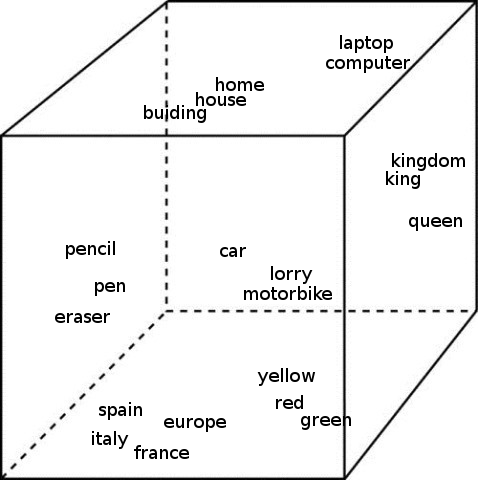
\includegraphics[width=0.5\textwidth]{img/words-cube.png}
        \end{center}

\end{frame}

% Slide 8: Applications of Embeddings
\begin{frame}{Applications of Embeddings}
    \begin{itemize}
        \item \textbf{Text-based applications}:
        \begin{itemize}
            \item Sentiment analysis, machine translation, question answering, etc.
        \end{itemize}
        \item \textbf{Non-text applications}:
        \begin{itemize}
            \item Representing users (e.g., recommender systems).
            \item Representing products (e.g., in e-commerce search).
        \end{itemize}
        \item Advantages of embeddings:
        \begin{itemize}
            \item Compact and efficient representations.
            \item Capture semantic relationships between words or entities.
        \end{itemize}
    \end{itemize}
\end{frame}

\begin{frame}{Embeddings that represent sequences of words}
    \begin{itemize}
        \item \textbf{General-purpose sentence embeddings}: USE, SBERT, SimCSE.
        \item \textbf{Multilingual tasks}: LASER, Multilingual USE, XLM-RoBERTa.
        \item \textbf{Lightweight options}: MiniLM, DistilBERT.
        \item \textbf{Paragraph embeddings}: Doc2Vec, GPT-based models, T5.
    \end{itemize}
\end{frame}



% Slide 9: Distance Between Vectors
\begin{frame}{Distance Between Vector Representations}
    \begin{itemize}
        \item To compare two vector representations (e.g., for sentences or documents), we compute their \textbf{distance} or \textbf{similarity}.
        \item Common measures:
        \begin{itemize}
            \item \textbf{Euclidean Distance}: Measures the straight-line distance between vectors.
            \item \textbf{Cosine Similarity}: Measures the cosine of the angle between vectors in the vector space.
        \end{itemize}
        \item Why use cosine similarity?
        \begin{itemize}
            \item Focuses on orientation, not magnitude.
            \item Ideal for high-dimensional and sparse data (e.g., text embeddings).
        \end{itemize}
    \end{itemize}
\end{frame}

% Slide 10: Computing Cosine Similarity
\begin{frame}{Computing Cosine Similarity}
    \begin{itemize}
        \item \textbf{Formula for Cosine Similarity}:
        \[
        \text{cosine similarity} = \frac{\vec{u} \cdot \vec{v}}{\|\vec{u}\| \|\vec{v}\|}
        \]
        Where:
        \begin{itemize}
            \item \(\vec{u} \cdot \vec{v}\) = dot product of the two vectors.
            \item \(\|\vec{u}\|\) and \(\|\vec{v}\|\) = magnitudes (norms) of the vectors.
        \end{itemize}
        \item \textbf{Steps}:
        \begin{enumerate}
            \item Compute the dot product: \(\vec{u} \cdot \vec{v} = \sum_{i=1}^{n} u_i v_i\)
            \item Compute the magnitudes: \(\|\vec{u}\| = \sqrt{\sum_{i=1}^{n} u_i^2}, \|\vec{v}\| = \sqrt{\sum_{i=1}^{n} v_i^2}\)
            \item Divide the dot product by the product of magnitudes.
        \end{enumerate}
        \item \textbf{Result}:
        \begin{itemize}
            \item Value ranges from -1 (opposite) to +1 (identical).
            \item A higher value means higher similarity.
        \end{itemize}
    \end{itemize}
\end{frame}

\section{Concluding remarks}

\begin{frame}{CL vs NLP}
    \begin{itemize}
        \item Computational Linguistics (CL) and Natural Language Processing (NLP) are closely related, yet distinct fields.
        \item CL provides the theoretical foundation, while NLP focuses on practical implementation and real-world applications.
        \item Both fields are crucial for advancing our understanding of human language and improving human-computer interactions.
        \item Many of the tasks analyzed today are useful in these two disciplines.
    \end{itemize}
\end{frame}

\begin{frame}{Text preprocessing}
    \begin{itemize}
        \item Crucial first step in NLP pipelines, ensuring data is clean, consistent, and ready for analysis.
        \item Key sub-tasks include removing formatting, tokenization, and normalization, each contributing to better model performance.
        \item Effective preprocessing requires tailored techniques for different tasks and languages.
    \end{itemize}
    \vspace{1em}
\end{frame}

\begin{frame}{Morphological parsing}
    \begin{itemize}
        \item Very relevant in CL, as it allows word-level analysis of corpora, and helps to understand and identify linguistic phenomena.
        \item Especially relevant for low-resourced languages, for which it still plays a relevant role in NLP.
        \item Essential for handling rich morphology, reducing vocabulary size, and improving NLP models.
        \item Unimorph and Universal Dependences are two of the most relevant multilingual resources for this task.
    \end{itemize}
\end{frame}

\begin{frame}{Syntactic parsing}
    \begin{itemize}
        \item Aimed at understanding the structure and relationships between words in a sentence.
        \item Both phrase structure and dependency structure provide valuable insights, with dependency structure being more flexible across languages.
        \item Syntax remains important in NLP, especially for low-resource languages, aiding tasks like disambiguation, summarization, and named entity recognition.
        \item The use of universal dependencies and parsing tools like Stanza and ScyPy enhances syntactic analysis in a multilingual context.
    \end{itemize}
\end{frame}

\begin{frame}{Vector representations of text}
    \begin{itemize}
        \item Words have complex relationships based on meaning: synonymy, antonymy, similarity, relatedness, etc.
        \item These relationships are fundamental to how we represent and understand language computationally.
        \item Vector semantics allow to represent word meanings as numeric vectors in high-dimensional spaces.
        \item Methods like \textbf{Bag-of-Words} and \textbf{TF-IDF} provide basic yet powerful representations for text; embeddings capture more nuanced semantic relationships.
        \item Comparing vector representations, such as through \textbf{cosine similarity}, enables efficient comparison of texts and supports a wide range of NLP applications.
    \end{itemize}
\end{frame}


\end{document}
